%========================================================================================
% TU Dortmund, Informatik Lehrstuhl VII
%========================================================================================

\chapter{Rendering}
\label{Kapitel 2}
%

\section{Partikelsystem}
\label{Kapitel_2_-_Unterkapitel_1}
%
Partikelsysteme sind in interaktiven Anwendungen wie Computerspiele und in der Postproduktion von Filmen, seien es Real- oder Animationsfilme, allgegenwärtig.
Man denke an typische Effekte wie Feuer und Rauch, aber auch Flüssigkeiten lassen sich mithilfe von Partikelsystemen realisieren.

In seinem im Jahre 1983 veröffentlichtem Papier(siehe \cite{reeves:particle_systems}) bezeichnet William T. Reeves diese Arten von Objekten als ‚fuzzy‘. Erstens sind sie zu komplex, um sie als Ganzes mit einem einzigen Mesh darstellen zu können. Daher teilt man das gesamte Objekt in viele kleinere Objekte, also die typischen Primitive wie Punkte, Linien oder Dreiecke. Zweitens bleibt die Form dieser Objekte meistens nicht starr, sie ändert sich im Verlauf der Zeit. Man denke beispielsweise an die Ausbreitung von Rauch. Drittens ist die Ausbreitung der Partikel keinem deterministischem Prozess unterworfen.

In unserer Anwendung wird ein Partikelsystem genutzt um den Flugverlauf des Balles darzustellen. 

\subsection{Komponenenten des Partikelsystems}
\label{Kapitel_2_-_Unterkapitel_1.1}
%
In der Anwendung besteht das Partikelsystem aus zwei Klassen, nämlich dem {\texttt{Particle}} und dem {\texttt{BallParticleRenderable}}.\\
Die {\texttt{Particle}} Klasse repräsentiert ein Partikel, welches eine Position in Weltkoordinaten, eine Geschwindigkeit, eine Lebensdauer und eine Größe hat. 
Die {\texttt{BallParticleRenderable}} Klasse ist für die Darstellung und Verwaltung aller im System vorhandenen Partikel zuständig. Zur Verwaltung gehört das emittieren neuer Partikel, das Aktualisieren der aktiven Partikel und Löschen der ‚toten‘ Partikel, also solcher, deren Lebensdauer null erreicht hat. Die Klasse hält Attribute, die die maximale Anzahl der aktiven Partikel beschränkt sowie die Emittiergeschwindigkeit.  Sie hat auch ein Attribut für die Position. Alle neuen Partikel werden relativ zu dieser Position emittiert. Dabei ist die Position des Emittierpunktes auf dem Rand des Balles entgegengesetzt dem Geschwindigkeitsvektor des Balles.

\subsection{Instanced Rendering}
\label{Kapitel_2_-_Unterkapitel_1.2}
%
Instanced Rendering bezeichnet eine effiziente Variante des Renderns von Objekten die dieselben Renderdaten, also dasselbe Mesh, verwenden, sich aber nur darin unterscheiden wo sie im Weltkoordinatensystem platziert werden. Für die Partikel unseres Partikelsystem trifft dies zu, da jedes Partikel in der Szene als Quad, bestehend aus 6 Vertices, dargestellt wird, auf das eine Textur projiziert wird.

Üblicherweise führt man in OpenGL ein Draw-Call durch den Aufruf der Funktion {\texttt{glDrawArrays}} oder {\texttt{glDrawElements}} aus. Um alle aktiven Partikel zu rendern würde man in jedem Frame über die Partikelliste iterieren und für jedes Partikel eine der eben genannten Funktionen aufrufen. Das Problem hierbei ist, das ein häufiges Aufrufen dieser Funktionen zu einem Performanceverlust führt, da die Befehle über den langsamen Peripheriebus zur Grafikkarte gesendet werden müssen. OpenGL bietet mit den Funktionen {\texttt{glDrawArraysInstanced}} und {\texttt{glDrawElementsInstanced}} die Möglichkeit mehrere Instanzen desselben Modells mit nur einem Funktionsaufruf zu rendern.

Aufgrund von Beschränkungen in GLSL ist es nicht möglich ein beliebig großes Array an Model-Matrizen als Uniform-Variable an den Vertexshader zu senden. Daher werden die Model-Matrizen in einem Array-Buffer gespeichert, welcher in jedem Frame aktualisiert werden muss, da sich die Anzahl der Partikel und ihre Positionen mit jedem Frame ändert. 
Um Instanced Rendering zu nutzen müssen die Model-Matrizen noch als Instance-Variablen deklariert werden. Dies geschieht mit dem Aufruf der Funktion glVertexAttribDivisor, die zwei Parameter hat. Der erste Parameter gibt die Speicheradresse der Variable im Vertexshader-Programm an und der zweite Parameter gibt an wann der nächste Wert aus der Instance-Variablen geholt wird. Der zweite Parameter muss ein Wert ungleich Null sein.  Der Aufruf der Funktion sollte bei der Assoziation der Array-Buffer mit den Variablen des Shader-Programms erfolgen, sprich nach dem Aufruf von glVertexAttribPointer.
Abbildung zeigt beispielhaft wie rendern mit instance-Variablen abläuft.
(Hier Abbildung + kurze Erklärung).

\subsection{Billboarding}
\label{Kapitel_2_-_Unterkapitel_1.3}
%
Für ein besseres visuelles Ergebnis werden die Quads, auf die die Partikeltextur projiziert werden, immer orthogonal zur Blickrichtung der Kamera gerendert. Die Quads erfahren durch die
Modelview-Matrix keinerlei Rotationen. Um diesen Effekt, der als Billboarding bezeichnet wird, zu erreichen muss der Rotationsanteil der View-Matrix, also die linke obere 3x3-Matrix, auf die Einheitsmatrix gesetzt werden.

(Hier Abbildung ohne Billboarding)

Rotationsmatrizen sind Orthogonalmatrizen, das heißt, dass ihre Inversen ihren Transponierten entsprechen. Es genügt also beim Berechnen der Modelview-Matrix die obere linke 3x3-Matrix der Model-Matrix durch die Transponierte des Rotationsanteils der View-Matrix zu ersetzen. Da die Partikel in unserem System auch eine Größe haben wird die
resultierende ModelView-Matrix noch mit einer Skalierungsmatrix multipliziert werden.

\subsection{Blending und Tiefentest}
\label{Kapitel_2_-_Unterkapitel_1.4}
%
In dem verwendeten Partikelsystem sollen die Farben der Partikel, wenn sie sich überlagern, addiert werden. Der resultierende Effekt ist, dass bei genügend sich überlagernden Partikel ein leuchtend weißer Bereich zu sehen ist. Blending erlaubt es, Farben miteinander zu vermischen und ist ein Teil der Verarbeitung der Fragmente in der Rendering Pipeline. OpenGL bietet verschiedene Blending-Arten an, die durch den Aufruf der Funktion {\texttt{glBlendFunc}} eingestellt werden können. 

\begin{figure}[h]
\centering
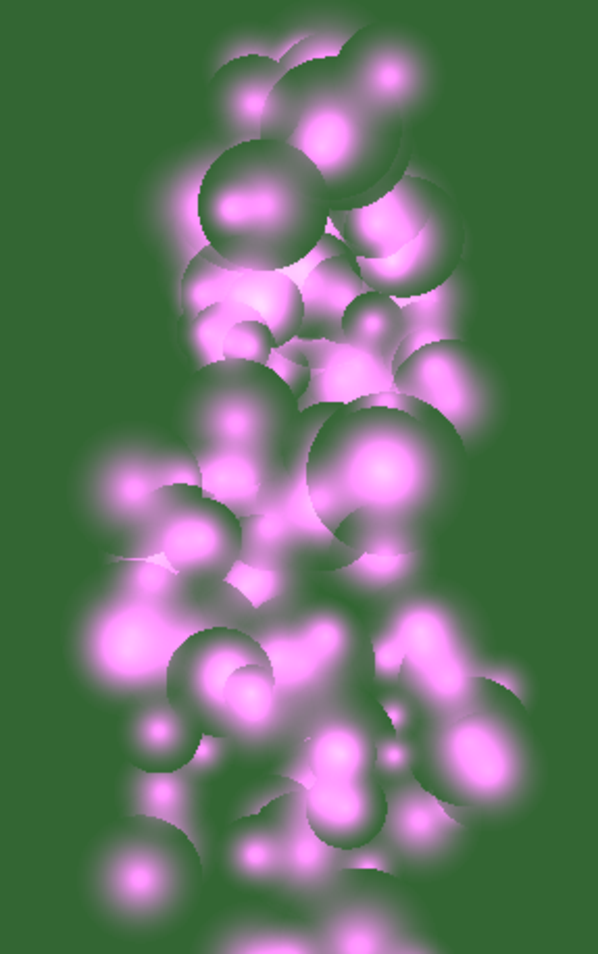
\includegraphics[scale=0.4]{bilder/BlendingEnabled}
\caption{Partikelsystem bei aktiviertem Blending}
\label{fig:BlendingEnabled}
\end{figure}

Abbildung 2.1 zeigt wie das Partikelsystem bei eingeschaltetem Blending und Verwendung von {\texttt{glBlendFunc}} mit den Argumenten {\texttt{GL\_SRC\_ALPHA}} und {\texttt{GL\_ONE}} aussieht. Eine Übersicht über die verschiedenen Argumente für {\texttt{glBlendFunc}} und ihre Auswirkungen auf die Farbe eines Fragments ist in \cite{virag:2012} zu finden.

Wie an Abbildung 2.1 zu erkennen ist tritt trotz eingeschaltetem Blending der gewünschte Effekt nicht auf. Grund dafür ist der Tiefentest. Für den Tiefentest spielt es keine Rolle, ob ein Fragment teilweise transparent ist, da der Tiefenwert für ein Fragment trotzdem in den Tiefenpuffer geschrieben wird, vorausgesetzt der Wert ist geringer.

Um dies zu umgehen, lässt sich mittels der Funktion {\texttt{glDepthMask}} das Schreiben in den Tiefenpuffer für das Rendern der Partikel verbieten.
Das endgültige Resultat ist in Abbildung 2.2 zu sehen.

\begin{figure}[h]
	\centering
	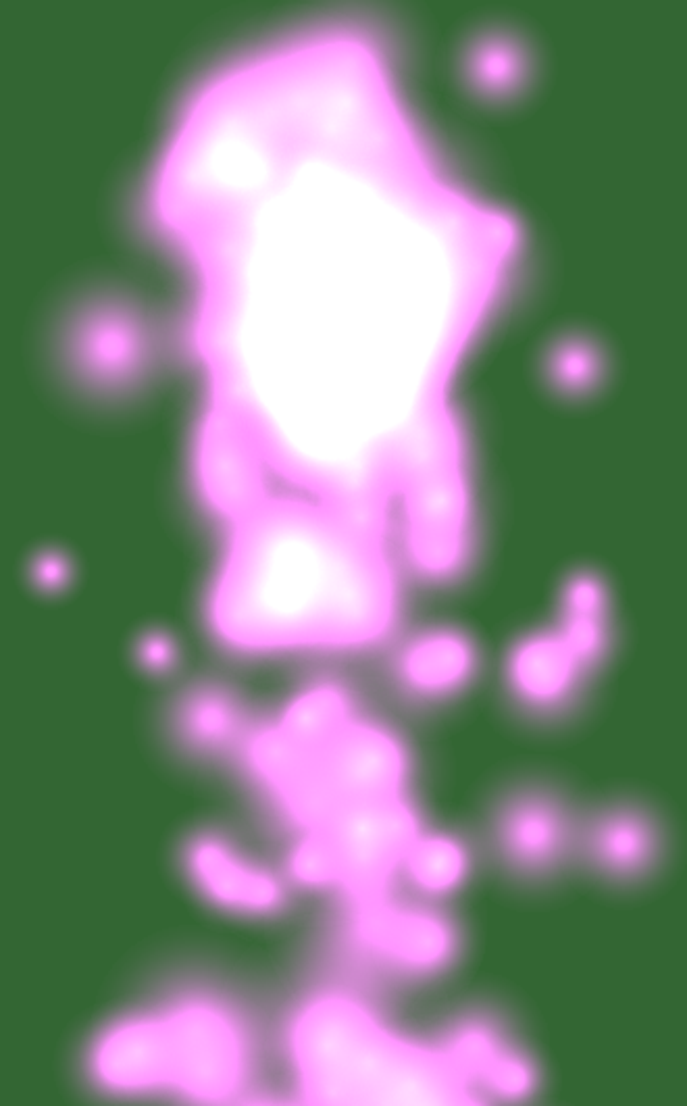
\includegraphics[scale=0.4]{bilder/ParticleFinal}
	\caption{Partikelsystem bei aktiviertem Blending und nicht-beschreibbarem Tiefenpuffer}
	\label{fig:ParticleFinal}
\end{figure}
%